Se tienen 4 ciudades unidas por 7 puentes. Encuentre una forma de dar un paseo, pasando por todos los puentes,
recorriendo solo una vez cada uno y regresando a la misma ciudad desde donde partiste.

\begin{center}

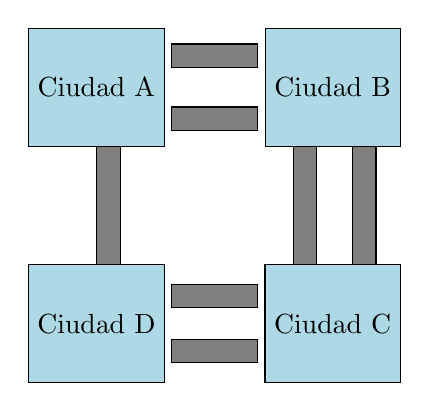
\begin{tikzpicture}

\centering
\definecolor{lightblue}{RGB}{173, 216, 230}

% Draw the cities
\node[draw, rectangle, minimum size=1.5cm, fill=lightblue] (A) at (0,0) {Ciudad A};
\node[draw, rectangle, minimum size=1.5cm, fill=lightblue] (B) at (3,0) {Ciudad B};
\node[draw, rectangle, minimum size=1.5cm, fill=lightblue] (C) at (3,-3) {Ciudad C};
\node[draw, rectangle, minimum size=1.5cm, fill=lightblue] (D) at (0,-3) {Ciudad D};

% Draw the bridges as rectangles
\draw[fill=gray] (0.95,0.25) rectangle (2.05,0.55); % A to B
\draw[fill=gray] (0,-0.75) rectangle (0.3,-2.25); % A to D
\draw[fill=gray] (2.5,-0.75) rectangle (2.8,-2.25); % B to C
\draw[fill=gray] (0.95,-3.2) rectangle (2.05,-3.5); % C to D

% Additional bridges
\draw[fill=gray] (0.95,-0.25) rectangle (2.05,-0.55); % A to C
\draw[fill=gray] (0.95,-2.5) rectangle (2.05,-2.8); % B to D
\draw[fill=gray] (3.25,-0.75) rectangle (3.55,-2.25); % B to C

\end{tikzpicture}
   
\end{center}